\documentclass[german,10pt,xcolor=colortbl,compress
%,draftrr
]{beamer}
\usepackage[utf8]{inputenc}
\usepackage[ngerman]{babel}
\usepackage{tabularx,ragged2e}

\usepackage{graphicx}
\graphicspath{{./img/}}

\usetheme{Copenhagen}  %% Themenwahl

\usecolortheme{seagull}


\title{Einstieg in die Akkreditierung}
\author{Daniela Kern-Michler, Philipp Jaeger}
\date{\today}

\def\bingo{
\footnotesize
  \begin{tabular}{|m{.2\textwidth}|m{.2\textwidth}|m{.2\textwidth}|m{.2\textwidth}|}
  %\begin{tabular}
  \hline
  Akkreditierungs\-verfahren & Hochschul\-rektorenkonferenz (HRK) & System\-akkreditierung & Akkreditierungs\-kriterien \\\hline
  Akkreditierungs\-entscheidung & L\"andergemein\-same Struktur\-vorgaben & Gutachter & Begehung \\\hline
  Akkreditierungs\-agentur & Akkreditierungs\-rat (AR) & Modul & European Credit Transfer and Accumulation System (ECTS) \\\hline
  Modulabschluss\-pr\"ufung & Pr\"ufungs\-leistung & Studien\-leistung & Kultusminister\-konferenz (KMK) \\\hline
  Studienakkredi\-tierungsstaats\-vertrag\newline (StAkkrStV) & Musterrechts\-verordnung (MRVO) &  Gutachten & Programm\-akkreditierung \\\hline
  \end{tabular}
}

\begin{document}
\begin{frame}
\maketitle
\vfill
\hspace*{.8\linewidth}
\includegraphics[width=2cm]{CC-BY-SA.png}
\end{frame}


\begin{frame}
\tableofcontents
\end{frame}

\section[Akkreditierung]{Akkreditierung? Akkreditierung!}

\frame{\tableofcontents[currentsection]}
%%%%%%%%%%%%%%%%%%%%%%%%%%%%%%%%%%%%%%%%%%%%%%%%%%%%%%%%%%%%%%%
\begin{frame}
  \frametitle{Was ist Akkreditierung?}
  \begin{itemize}
  	\item Prüfverfahren für Studiengänge
  	\item eine Art ``TÜV`` oder Qualitätssiegel
  	\item legt Mindeststandards fest
  	\item prüft Studierbarkeit
  	\vspace{1cm}
  	\item mittlerweile (und immer mehr) auch für Qualitätssicherungssysteme $\rightarrow$ Systemakkreditierung
  \end{itemize}   
\end{frame}
%%%%%%%%%%%%%%%%%%%%%%%%%%%%%%%%%%%%%%%%%%%%%%%%%%%%%%%%%%%%%%%
\begin{frame} 
  \frametitle{Historische Schlagwörter zur deutschen Entwicklung} 
  \begin{itemize}
  	\item Bologna-Erklärung 1999
  		\begin{itemize}
  			\item Harmonisierung des europäischen Hochschulsystems
  			\item Gemeinsame Qualitätssicherung
  		\end{itemize}
  	\pause
  	\item Regel zur Akkreditierung und Ländergemeinsame Strukturvorgaben
  	\item Studentenproteste/Bildungsstreiks führen zu Überarbeitungen
  	\item Beschluss des Bundesverfassungsgerichtes erklärt Regelungen in NRW für ungültig (2016)
  	\vspace{1cm}
  	\pause
  	\item \textbf{seit 1.1.2018: Akkreditierungsstaatsvertrag und Musterrechtsverordnung zur Akkreditierung sind rechtliche Grundlage}
  	\item Bundesländer erlassen Rechtsverordnungen
  \end{itemize}   
\end{frame}
%%%%%%%%%%%%%%%%%%%%%%%%%%%%%%%%%%%%%%%%%%%%%%%%%%%%%%%%%%%%%%%
\begin{frame} 
  \frametitle{Warum beschäftigen wir uns damit?} 
  \begin{itemize}
  	\item unsere Studiengänge durchlaufen die Verfahren
  		\begin{itemize}
  			\item Studierbarkeit wird zertifiziert
  			\item Aufmerksamkeit für Fragen zu Studium und Lehre
  		\end{itemize}
  	\pause
  	\item wir bringen die studentische Perspektive in die Prüfverfahren $\rightarrow$ Studentischer Akkreditierungspool
  	\pause
  	\item wir nehmen in Resos Stellung zum Akkreditierungssystem und seinen Veränderungen
  \end{itemize}   
\end{frame}
%%%%%%%%%%%%%%%%%%%%%%%%%%%%%%%%%%%%%%%%%%%%%%%%%%%%%%%%%%%%%%%
\begin{frame} 
  \frametitle{Akkreditierungsbingo} 
  \bingo
  %\includegraphics[width=1\textwidth]{akkreditierungs-bingo.png}
%\begin{tabular}{|p{0.22\textwidth}|p{0.22\textwidth}|p{0.22\textwidth}|p{0.22\textwidth}|}
%\hline
%Akkreditierungs-verfahren & Programm-akkreditierung & System-akkreditierung & Akkreditierungs-kriterien\\
%\hline
%Akkreditierungs-entscheidung & Gutachten & Gutachter & Begehung \\
%\hline
%Akkreditierungs-agentur & Akkreditierungs-rat & Modul & European Credit Transfer and Accumulation System (ECTS)\\
%\hline
%Modulabschluss-prüfung & Studienleistung & Prüfungsleistung & Kultusminister-konferenz (KMK)\\
%\hline
%Staatsvertrag & Musterrechts-verordnung & Länder-gemeinsame Strukturvorgaben & Hochschul-rektoren-konferenz (HRK)\\
%\hline
%\end{tabular}
\end{frame}
%%%%%%%%%%%%%%%%%%%%%%%%%%%%%%%%%%%%%%%%%%%%%%%%%%%%%%%%%%%%%%%
\section{Stationenarbeit}
\frame{\tableofcontents[currentsection]}
%%%%%%%%%%%%%%%%%%%%%%%%%%%%%%%%%%%%%%%%%%%%%%%%%%%%%%%%%%%%%%%
\begin{frame} 
  \frametitle{Ablauf Stationenarbeit} 
  \begin{itemize}
  	\item Kleingruppen (3-5 Leute)
  	\item 15 min pro Station (teilweise etwas knapp $\rightarrow$ Überblick gewinnen
  	\vspace{0.5 cm}
  	\item Stationen:
  	\begin{itemize}
  		\item Akkreditierungssystem
  		\item Akkreditierungsverfahren
  		\item Akkreditierungskriterien
  		\item Regeln für die Studiengangsgestaltung
  	\end{itemize}
  \end{itemize}   
\end{frame}
%%%%%%%%%%%%%%%%%%%%%%%%%%%%%%%%%%%%%%%%%%%%%%%%%%%%%%%%%%%%%%%
\begin{frame} 
  \frametitle{Akkreditierungsbingo} 
  %\includegraphics[width=1\textwidth]{akkreditierungs-bingo.png}
  \bingo
\end{frame}
%%%%%%%%%%%%%%%%%%%%%%%%%%%%%%%%%%%%%%%%%%%%%%%%%%%%%%%%%%%%%%%
\section{Nachbesprechung}
\frame{\tableofcontents[currentsection]}
%%%%%%%%%%%%%%%%%%%%%%%%%%%%%%%%%%%%%%%%%%%%%%%%%%%%%%%%%%%%%%%
\begin{frame}
\frametitle{Persönlicher Merkzettel}
Was sind die entscheidenden Dokumente für die Akkreditierung? Wo findet man Informationen?
\vspace{0.5cm}
\begin{itemize}
\item Staatsvertrag
\item Musterrechtsverordnung
\item Landesgesetze
\end{itemize}
\pause
\begin{itemize}
\item Website Akkreditierungsrat
\item Website Studentischer Akkreditierungspool
\end{itemize}
\pause
\begin{itemize}
\item Nationaler Qualifikationsrahmen (DQR)
\item Europäische Qualifikationsrahmen (EQR)
\item The Standards and guidelines for quality assurance in the European Higher Education Area (ESG)
\end{itemize}
\end{frame}
%%%%%%%%%%%%%%%%%%%%%%%%%%%%%%%%%%%%%%%%%%%%%%%%%%%%%%%%%%%%%%%
\begin{frame}
\frametitle{Persönlicher Merkzettel}
Wie ist das deutsche Akkreditierungssystem aufgebaut?
\vspace{0.5cm}
  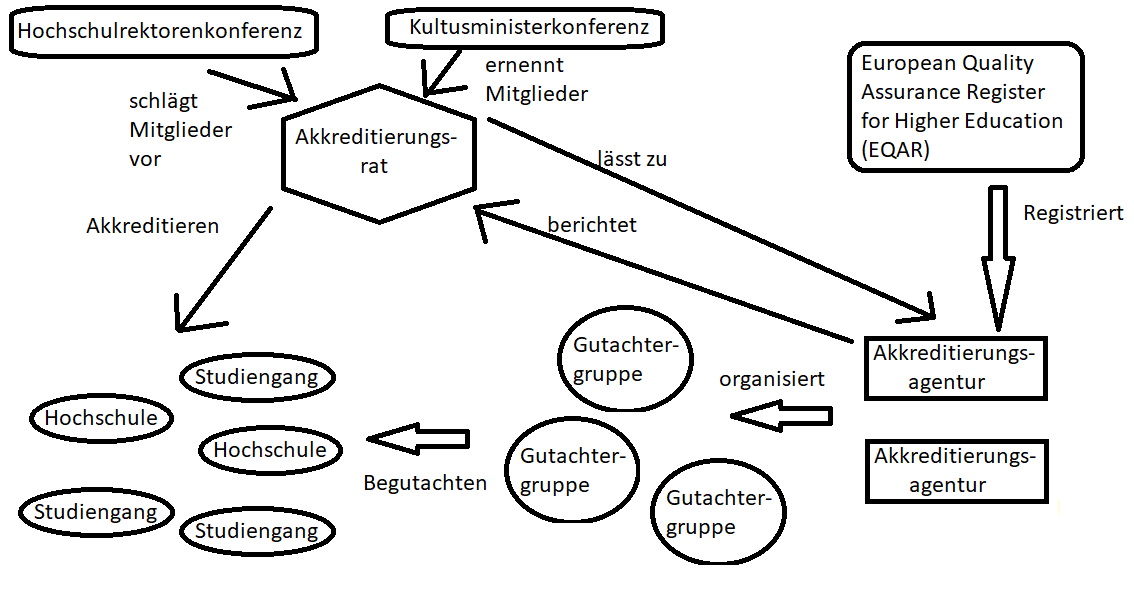
\includegraphics[width=1\textwidth]{Schaubild2.png}
\end{frame}
%%%%%%%%%%%%%%%%%%%%%%%%%%%%%%%%%%%%%%%%%%%%%%%%%%%%%%%%%%%%%%%
\begin{frame}
\frametitle{Persönlicher Merkzettel}
Wie ist das schweizer Akkreditierungssystem aufgebaut?
\begin{itemize}
\item Institutionelle Akkreditierung
\item Programmakkreditierung auf Wunsch
\item nur eine Agentur AAQ
\item Akkreditierungsentscheide durch Akkreditierungsrat
\item Hochschulförderungs- und Koordinationsgesetz (HFKG)
\end{itemize}
\pause
Wie ist das österreichische Akkreditierungssystem aufgebaut?
\begin{itemize}
\item Institutionelle Akkreditierung
\item nur eine Agentur AQA
\item Hochschul-Qualitätsicherungsgesetz (HS-QSG)
\end{itemize}
\end{frame}
%%%%%%%%%%%%%%%%%%%%%%%%%%%%%%%%%%%%%%%%%%%%%%%%%%%%%%%%%%%%%%%
\begin{frame}
\frametitle{Persönlicher Merkzettel}
Wie sieht ein Akkreditierungsverfahren aus?
\vspace{0.5cm}
  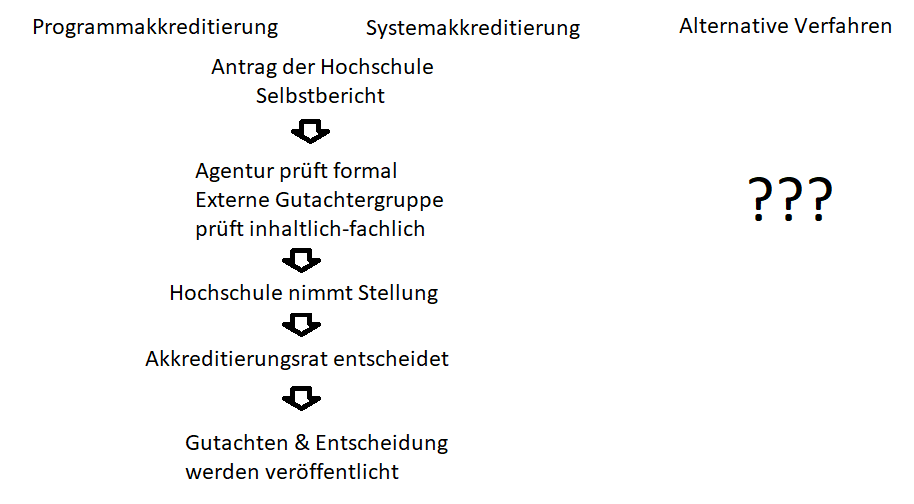
\includegraphics[width=1\textwidth]{verfahren.png}
Begutachtung muss nicht Vor-Ort Begehung bedeuten...
\end{frame}
%%%%%%%%%%%%%%%%%%%%%%%%%%%%%%%%%%%%%%%%%%%%%%%%%%%%%%%%%%%%%%%
\begin{frame}
\frametitle{Persönlicher Merkzettel}
Was wird geprüft?
\vspace{0.5cm}
\textbf{Formale Kriterien}
\begin{itemize}
\item Studienstruktur und -dauer
\item Studiengangsprofil
\item Zugangsvoraussetzungen und Übergänge
\item Abschlüsse und deren Bezeichnungen
\item Modularisierung
\item Leistungspunktesystem
\item ...
\end{itemize}
\end{frame}
%%%%%%%%%%%%%%%%%%%%%%%%%%%%%%%%%%%%%%%%%%%%%%%%%%%%%%%%%%%%%%%
\begin{frame}
\frametitle{Persönlicher Merkzettel}
Was wird geprüft?
\vspace{0.5cm}
\textbf{Fachlich-inhaltliche Kriterien}
\begin{itemize}
\item Qualifikationsziele und Abschlussniveau
\item Studiengangskonzept und Umsetzung
\item Fachlich-inhaltliche Gestaltung
\item Studienerfolg
\item Geschlechtergerechtigkeit und Nachteilsausgleich
\item ...
\end{itemize}
\end{frame}
%%%%%%%%%%%%%%%%%%%%%%%%%%%%%%%%%%%%%%%%%%%%%%%%%%%%%%%%%%%%%%%
\begin{frame}
\frametitle{Persönlicher Merkzettel}
Was für Akkreditierungsentscheidungen gibt es? Wie lange gelten sie?
\begin{itemize}
\item Akkreditierung und Nicht-Akkreditierung
\item Akkreditierung mit Auflagen (in der Regel in 12 Monaten nachzuweisen) \emph{künftig nur noch als Ausnahme?!}
\item Erstmalige Akkreditierung: 8 Jahre
\item Reakkreditierung: 8 Jahre
\item früher gab es noch das \emph{Aussetzten des Verfahrens}
\end{itemize}
\end{frame}
%%%%%%%%%%%%%%%%%%%%%%%%%%%%%%%%%%%%%%%%%%%%%%%%%%%%%%%%%%%%%%%
\section{Mitgestaltung}
\frame{\tableofcontents[currentsection]}
%%%%%%%%%%%%%%%%%%%%%%%%%%%%%%%%%%%%%%%%%%%%%%%%%%%%%%%%%%%%%%%
\begin{frame}
\frametitle{Studentischer Akkreditierungspool}
Stellt studentische Vertretung:
\begin{itemize}
\item in Gutachtergruppen bei Programm- und Systemakkreditierung
\item im Akkreditierungsrat
\item als die Agenturen noch entschieden haben auch in Kommissionen dort
\end{itemize}
Organisiert:
\begin{itemize}
\item Vernetzungstreffen
\item \textbf{Schulungsseminare}
\end{itemize}
\hspace*{7cm}
\includegraphics[scale=0.6]{pool.PNG}
\end{frame}
%%%%%%%%%%%%%%%%%%%%%%%%%%%%%%%%%%%%%%%%%%%%%%%%%%%%%%%%%%%%%%%
\begin{frame}
\frametitle{Studentischer Akkreditierungspool}
Mitglieder werden entsendet von:
\begin{itemize}
\item Bundesfachschaftentagungen
\item fzs (freier zusammenschluss von studentInnenschaften)
\item Landes-Asten-Konferenzen
\end{itemize}
\hspace*{7cm}
\includegraphics[scale=0.6]{pool.PNG}
\end{frame}
%%%%%%%%%%%%%%%%%%%%%%%%%%%%%%%%%%%%%%%%%%%%%%%%%%%%%%%%%%%%%%%
\begin{frame}
\frametitle{Andere Orte der Mitwirkung}
An Euren Hochschulen:
\begin{itemize}
\item Gremien auf unterschiedlichen Ebenen: Qualitätszirkel, Akkreditierungskommissionen, Studienkommissionen, teilweise Prüfungskommissionen...
\item Erstellung des Selbstberichtes
\item Vor-Ort Begehung
\item evtl. Stellungnahme vor Akkreditierungsentscheidung
\end{itemize}
\vspace*{0.5cm}
Auf der ZaPF...
\end{frame}
%%%%%%%%%%%%%%%%%%%%%%%%%%%%%%%%%%%%%%%%%%%%%%%%%%%%%%%%%%%%%%%
\section[ZaPF]{Positionen der ZaPF}
\frame{\tableofcontents[currentsection]}
%%%%%%%%%%%%%%%%%%%%%%%%%%%%%%%%%%%%%%%%%%%%%%%%%%%%%%%%%%%%%%%
\begin{frame}
\frametitle{ZaPF \& Akkreditierung}
Manchmal etwas unübersichtlich und ein Thema auf dieser ZaPF, aber schon einiges an Arbeit.\\ 

Relevant für Akkreditierungsverfahren:
\begin{itemize}
\item Wikiseite: Kategorie:Akkreditierung (zu finden unter Themen und Projekte)
\item Richtlinien für Bachelor- und Masterstudiengänge (WiSe 2008)
\item Positionspapier und Resolution zur Ausgestaltung von Qualitätsmanagementsystemen (WiSe 2012 und SoSe 2013)
\item Positionspapier der ZaPF zum studentischen Akkreditierungspool (SoSe 2012)
\end{itemize}

\end{frame}
%%%%%%%%%%%%%%%%%%%%%%%%%%%%%%%%%%%%%%%%%%%%%%%%%%%%%%%%%%%%%%%
\begin{frame}
\frametitle{ZaPF \& Akkreditierung}

Relevant für Arbeit auf der ZaPF:
\begin{itemize}
\item Alles, was jemals beschlossen oder beredet wurde ;-)
\item Protokoll AK Überarbeitung der Akkreditierungsrichtlinien (WiSe 2015)
\item Positionspapier und Reso zur Akkreditierung (Änderungen der Gesetzeslage)(WiSe 2017)
\item Positionspapier zum deutschen Akkreditierungssystem (SoSe 2016)
\end{itemize}
\vspace{0.5cm}
Fleißig ins Wiki schauen, um doppelte Arbeit zu vermeiden!\\
$\rightarrow$ Akkreditierung I \& Akkreditierung II
\end{frame}
%%%%%%%%%%%%%%%%%%%%%%%%%%%%%%%%%%%%%%%%%%%%%%%%%%%%%%%%%%%%%%%
\section*{Fragen}
\begin{frame}
\centering
\Large{ Fragen?}
\end{frame}
\end{document}
